\documentclass[10.3pt,a4paper]{article}
\usepackage[margin=18mm]{geometry}
\usepackage{kotex,fontspec}
\setmainfont{Noto Sans CJK KR}
\setsansfont{Noto Sans CJK KR}
\setmonofont{DejaVu Sans Mono}
\usepackage{amsmath,amssymb,bm,mathtools}
\usepackage{booktabs,tabularx,longtable,array,makecell,multirow}
\usepackage{enumitem,setspace,xcolor,hyperref,cleveref}
\usepackage{tikz}
\usetikzlibrary{arrows.meta,positioning,fit,calc,matrix}
\usepackage[most]{tcolorbox}
\usepackage{titlesec,caption,fancyhdr}
\usepackage[backend=biber,style=numeric,sorting=none,natbib=true,maxbibnames=20]{biblatex}
\addbibresource{references.bib}
\definecolor{Line}{HTML}{555555}
\definecolor{Panel}{HTML}{F4F4F4}
\definecolor{Core}{HTML}{ECEFF2}
\definecolor{Theory}{HTML}{EFF1EA}
\definecolor{Future}{HTML}{F3EEE8}
\hypersetup{colorlinks=true,linkcolor=black,citecolor=black,urlcolor=black}
\setstretch{1.18}
\setlength{\parindent}{0pt}
\setlength{\parskip}{4.2pt}
\setlength{\emergencystretch}{2em}
\setlist{nosep,leftmargin=1.5em}
\titleformat{\section}{\Large\bfseries}{\thesection.}{0.5em}{}
\titleformat{\subsection}{\large\bfseries}{\thesubsection.}{0.45em}{}
\pagestyle{fancy}\fancyhf{}
\lhead{CATENA v6.2 연구계획}\rhead{Transactional Control Algebra}\cfoot{\thepage}
\newtcolorbox{keybox}[1][]{colback=Panel,colframe=Line,boxrule=.45pt,arc=1.2mm,left=2.5mm,right=2.5mm,top=1.8mm,bottom=1.8mm,#1}
\newtcolorbox{claimbox}[1][]{colback=Core,colframe=Line,boxrule=.45pt,arc=1.2mm,left=2.5mm,right=2.5mm,top=1.8mm,bottom=1.8mm,#1}
\newtcolorbox{resultbox}[1][]{colback=Theory,colframe=Line,boxrule=.45pt,arc=1.2mm,left=2.5mm,right=2.5mm,top=1.8mm,bottom=1.8mm,#1}
\newcommand{\R}{\mathbb{R}}
\newcommand{\E}{\mathbb{E}}
\newcommand{\vect}[1]{\operatorname{vec}(#1)}
\newcommand{\op}[1]{\texttt{#1}}
\newcommand{\mse}{\operatorname{MSE}}

\begin{document}
\begin{center}
{\LARGE\bfseries CATENA: Transactional Control Algebra}\par{\LARGE\bfseries for Finite and Recurrent Memory}\par\vspace{3mm}
{\large 완료된 control-geometry evidence에서 learned operator와 sequence memory로}\par\vspace{4mm}
{\normalsize 연구계획서 v6.2 -- post-core expansion}\par\vspace{2mm}
{\small 2026년 7월 27일}
\end{center}

\begin{keybox}
\textbf{중심 질문.} 환경이 요구하는 update-demand family의 geometry와 algebra가, finite 또는 recurrent memory가 제공해야 할 최소 control rank, basis, address freedom과 state conditioning을 예측하는가? 그리고 controlled probe에서 확인된 원리가 representation과 update가 함께 학습되는 event-sequence memory에서도 유지되는가?
\end{keybox}

\section*{요약}
CATENA의 초기 목표는 외부 canonical state가 바뀐 뒤 stale internal state를 낮은 비용으로 동기화하는 것이었다. 그러나 compact patch 자체는 KV-cache editing과 latent-state injection 연구와 빠르게 인접해졌다\citep{kveraser2026}. 이에 연구의 중심을 patch interface에서 \textbf{transactional memory control의 구조적 조건}으로 이동했다. 완료된 H1--H4 controlled experiments는 네 가지 결과를 제공한다. 첫째, bounded behavioral reachability가 operation identity를 제거한 unseen-geometry error를 $R^2=0.9976$으로 예측했다. 둘째, erase와 write의 독립적인 magnitude control은 tied control이 갖는 asymmetric update error를 독립 OOD geometry에서 제거했다. 셋째, shared diagonal control의 충분성은 demand family의 joint diagonalizability로 결정되었고, graded JD regret는 held-out application error를 $R^2=0.999998$로 calibration했다. 넷째, dose, transplant, rescue와 scalarization intervention이 operation-specific control function과 architecture gap을 기능적으로 매개했다. Semantic front-end factorization은 두 번의 prospectively locked design gate에서 practical benefit를 열지 못했으며, 이는 semantic inference와 downstream memory controllability가 별도 병목임을 보여준다.

다음 연구는 같은 synthetic result를 더 반복하지 않는다. (E10) learned low-rank control이 best-rank reachable floor를 실제로 따라가는지, (E11) shared representation을 함께 학습해도 noncommuting demand의 obstruction이 남는지, (E12) magnitude, granularity, address, state-conditioning 자유도가 각각 필요한 demand family에서만 선택적 이득을 보이는지, (E13) 이러한 원리가 여러 update와 distractor를 포함한 structured event sequence로 전이되는지, (E14) update 전에 형성된 plan state를 수정할 수 있는지를 검증한다. E15는 official GDN2/KDA와 KVEraser를 별도 환경에서 엄격히 pinning하고, E16은 완료 evidence를 단일 registry로 동결한다. REALM 제출은 H1--H4 controlled core로 독립적으로 완결되며, post-core 결과는 통과한 경우에만 제한된 확장 evidence로 추가한다.

\tableofcontents
\newpage

\section{연구의 현재 위치}
\subsection{문제의 재정의}
Finite recurrent memory는 과거를 고정 크기 state에 압축한다. 외부의 verified transaction이 현재 규칙, 권한, preference 또는 tool state를 바꾸면 내부 memory는 다음 세 작업을 동시에 수행해야 한다.
\[
\text{stale influence 제거}
+\text{new association 기록}
+\text{unrelated content 보존}.
\]
GDN2는 delta-rule memory에서 erase와 write를 분리하며 tied scalar restriction을 제거한다\citep{gdn22026}. KDA와 GDN2를 공통 recurrent-memory notation으로 비교한 연구는 optimizer, stack 구성과 throughput을 포함한 multi-objective trade-off를 보여준다\citep{mechanisms2026}. CARVE는 stored content를 보는 state-conditioned gating을 도입하고\citep{carve2026}, EDA는 erase와 write의 address freedom을 분리한다\citep{eda2026}. Transformer에서는 KVEraser가 이미 처리된 span의 KV influence를 localized steering states로 제거한다\citep{kveraser2026}.

따라서 CATENA는 최초의 erase gate, state editing 또는 controllability analysis를 주장하지 않는다. 정확한 연구 공백은 다음이다.

\begin{claimbox}
\textbf{Novelty locus.} Verified update demand가 요구하는 geometry/algebra와 memory-control operator의 bounded behavioral reachable set을 같은 좌표계에서 정의하고, 그 불일치가 error, architecture interaction과 intervention sensitivity를 예측하는지 검증한다. 이어서 이 설계 원리가 learned representation, learned low-rank operator와 repeated event sequence에서도 유지되는지를 시험한다.
\end{claimbox}

\subsection{Demand algebra}
Transaction $\tau$가 요구하는 ideal update operator를 $P_\tau$라 하고, demand family $\mathcal T$가 생성하는 algebra를
\[
\mathcal A_{\mathcal T}=\operatorname{alg}\{P_\tau:\tau\in\mathcal T\}
\]
로 둔다. 이 algebra의 구조는 필요한 controller class에 대한 예측을 준다.

\begin{center}
\begin{tabularx}{\textwidth}{lXl}
\toprule
Demand property & 의미 & 최소 후보 control \\
\midrule
1차원 tied demand & erase와 write가 항상 같은 magnitude로 움직임 & tied scalar \\
독립 magnitude & erase-only, write-only corner가 존재 & dual scalar \\
공통 diagonal basis & family가 하나의 basis에서 jointly diagonalizable & shared diagonal \\
Noncommuting family & 하나의 shared diagonal basis로 표현 불가 & block/low-rank/matrix \\
Different erase/write address & 제거 위치와 기록 위치가 다름 & separate address \\
State-dependent target & 동일 observation이 stored content에 따라 다른 update 요구 & state-conditioned control \\
\bottomrule
\end{tabularx}
\end{center}

이 표는 architecture를 보편적으로 순위화하지 않는다. 추가 freedom은 그것을 요구하는 demand에서만 이득을 보여야 하며, 더 단순한 demand에서는 equivalence 또는 non-inferiority를 유지해야 한다.

\section{완료된 증거와 현재 claim ceiling}
\subsection{H1: Bounded behavioral reachability}
Finite state를 $S$, transaction을 $\tau$, controller variable을 $g\in\mathcal G$, update map을 $U(S,\tau,g)$라 둔다. Ideal target은 $S^\star=S+\Delta S^\star$다. Confirmatory predictor는 affected와 unaffected readout을 포함한 bounded behavioral regret다.
\[
R_{\mathrm{beh}}^2=
\min_{g\in\mathcal G}
\frac{1}{D_W}
\left\|W\left(U(S,\tau,g)-S^\star\right)\right\|_2^2.
\]
Operation fixed effect를 제거한 unseen geometry에서 $R_{\mathrm{beh}}^2$는 learned error를 $R^2=0.997615$로 예측했고 slope는 $1.008633$이었다. State feasible/span predictor보다 각각 약 0.0203, 0.0222 높은 OOS $R^2$를 보였다. 이는 nominal parameter 수보다 \textbf{행동적으로 도달 가능한 bounded update set}이 error floor를 더 직접적으로 설명함을 의미한다.

\subsection{H2: Erase/write factorization}
Oracle candidate/address 조건에서 tied와 dual controller는 동일 two-output head를 사용하고, tied condition만 diagonal subspace로 projection한다.
\[
(\tilde e,\tilde w)\mapsto
\left(\frac{\tilde e+\tilde w}{2},\frac{\tilde e+\tilde w}{2}\right).
\]
원본 E02는 \op{SUPERSEDE}의 tied-to-oracle headroom이 수치적으로 0이어서 relative equivalence가 정의되지 않아 \emph{inconclusive}로 보존했다. 사전에 absolute-equivalence repair를 동결한 E02b는 새로운 norm-angle OOD geometry에서 6/6 gate를 통과했다. ADD/INVALIDATE normalized gain은 0.999999760, asymmetric-symmetric interaction은 0.016343185, retention difference의 upper CI는 non-inferiority margin 안에 있었다. 따라서 허용되는 claim은 다음이다.

\begin{resultbox}
\textbf{H2 result.} Oracle candidate/address finite-memory setting에서 independent erase/write magnitude는 tied control의 asymmetric error를 제거하며, symmetric operation과 unrelated retention을 보존한다. 원본 E02의 inconclusive 판정은 변경하지 않는다.
\end{resultbox}

\subsection{H3: Joint diagonalizability}
Demand operator family가 shared basis $Q$에서 diagonalizable한지 다음 regret로 측정한다.
\[
R_{\mathrm{JD}}=
\min_{Q^\top Q=I}
\sum_{\tau}
\left\|\operatorname{offdiag}(Q^\top P_\tau Q)\right\|_F^2.
\]
원본 E03은 categorical contrast를 모두 통과했지만 nonzero predictor range가 좁아 global calibration gate가 실패했다. 이를 그대로 보존하고, application result를 보기 전에 analytic predictor로 6개 bin을 층화한 E03b를 별도 실행했다. 48개 family mean에서 calibration $R^2=0.999998169$, slope $1.000258921$, intercept $1.8464\times10^{-7}$이었다. 따라서 common rotation은 learned shared basis로 흡수되지만 noncommuting family는 shared diagonal class에 residual을 남긴다는 categorical/quantitative 결과가 함께 열린다.

\subsection{H4: Functional mediation}
E02 checkpoint 8쌍을 freeze하고 같은 $S,A,B$에서 operation만 바꾼 counterfactual quartet에 intervention을 적용했다. Primary relevant-minus-irrelevant interaction은 0.0312500, transplant cross-minus-same은 0.0624817, rescue cross-minus-same은 0.0312408이었다. 32/32 relevant dose curve가 단조적이었고, post-hoc scalarization은 tied-dual gap 0.015625의 99.9999906\%를 재현했다. Retention damage와 norm mismatch는 사실상 0이었다.

\begin{resultbox}
\textbf{H4 result.} Erase/write factorization의 architecture gap은 corresponding control을 제거하거나 scalarize할 때 재현되고, same-operation transplant/rescue에서만 회복된다. 이는 oracle-controlled finite memory 안에서 operation-specific functional mediation을 지지한다.
\end{resultbox}

\subsection{H5 boundary: semantic front-end factorization}
두 차례 prospective design gate에서 leakage, wrong-address, namespace와 parameter/compute control은 통과했으나 practical claim은 열리지 않았다. E05a-R1의 factorized/shared affected MSE는 각각 $2.366\times10^{-5}$, $3.547\times10^{-5}$로 둘 다 oracle floor에 가까웠다. 평균 gain은 $1.18\times10^{-5}$로 등록 SESOI $10^{-3}$보다 약 85배 작았고 seed 방향은 7/8이었다.

이 결과는 semantic inference가 실패했다는 뜻이 아니다. 더 정확한 boundary는 다음이다.
\[
\boxed{
\text{shared semantic representation}
\rightarrow
\text{explicit update demand}
\rightarrow
\text{geometry-matched memory controller}
}
\]
Semantic front-end까지 erase/write branch로 factorize할 필요는 확인되지 않았지만, 실제 state를 수정하는 downstream control surface의 geometry는 중요했다. H5는 이번 제출에서 닫고 다시 threshold를 조정하지 않는다.

\begin{figure}[t]
\centering
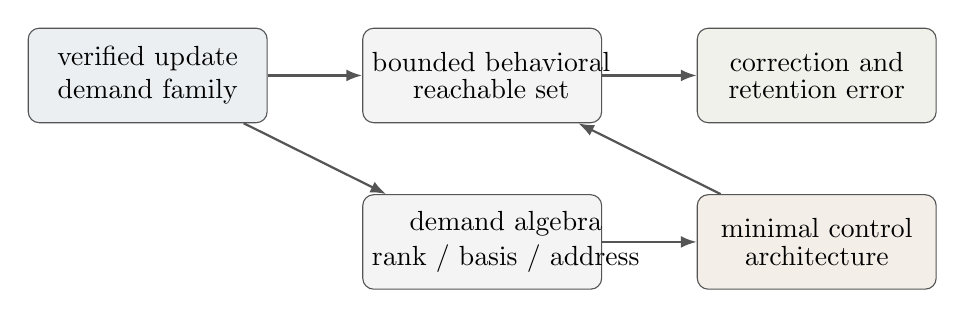
\begin{tikzpicture}[
 node distance=9mm and 12mm,
 b/.style={draw=Line,rounded corners=1.4mm,fill=Panel,minimum width=30mm,minimum height=12mm,text width=28mm,align=center},
 a/.style={-{Latex[length=2mm]},thick,draw=Line}
]
\node[b,fill=Core] (demand) {\shortstack{verified update\\demand family}};
\node[b,right=of demand] (reach) {\shortstack{bounded behavioral\\reachable set}};
\node[b,right=of reach,fill=Theory] (error) {\shortstack{correction and\\retention error}};
\node[b,below=of reach] (algebra) {\shortstack{demand algebra\\rank / basis / address}};
\node[b,right=of algebra,fill=Future] (arch) {\shortstack{minimal control\\architecture}};
\draw[a] (demand)--(reach);
\draw[a] (reach)--(error);
\draw[a] (demand)--(algebra);
\draw[a] (algebra)--(arch);
\draw[a] (arch)--(reach);
\end{tikzpicture}
\caption{완료된 core는 reachability와 control geometry를 검증했다. Post-core는 minimal control class를 학습하고 sequence-level persistence로 확장한다.}
\end{figure}

\section{Post-core 연구 가설}
\subsection{H6 / E10: Learned control-rank scaling}
\textbf{질문.} E03의 low-rank 결과는 oracle upper bound였다. 실제 transaction-conditioned rank-$r$ controller가 best-rank reachable floor를 학습하며, 필요한 최소 rank가 demand family의 intrinsic rank와 함께 증가하는가?

\textbf{데이터.} Descriptor $z\in\R^{16}$를 smooth coefficient로 변환하는 operator family
\[
P(z)=U\operatorname{diag}(c(z))V^\top
\]
를 생성한다. Intrinsic rank $r^\star\in\{1,2,4,8,16\}$, matrix dimension 64, train/test descriptor 4096/2048, 8 seeds를 사용한다. Test descriptors는 train과 분리한다.

\textbf{모델.} Learned rank $r\in\{1,2,4,8,16,32\}$의 low-rank controller
\[
\widehat P_r(z)=L_\theta(z)R_\theta(z)^\top.
\]
각 $r$에 대해 best rank-$r$ SVD oracle을 함께 계산한다.

\textbf{학습.} 4,000 steps, batch 256, AdamW, LR $10^{-3}$, weight decay $10^{-4}$. Loss는 entrywise matrix MSE다.

\textbf{Primary metrics.}
\begin{itemize}
\item held-out operator MSE와 best-rank oracle 대비 excess error;
\item baseline-to-oracle headroom 중 learned model이 회복한 비율;
\item quality threshold를 최초로 통과하는 learned rank $r_{\min}$;
\item rank별 parameter, active coefficient와 MACs.
\end{itemize}

\textbf{Gate.} $r_{\min}\le2r^\star$인 cell 비율 0.8 이상, rank 증가에 따른 error 단조성 0.9 이상, low-rank 대 high-rank seed sign-flip $p\le0.05$. 통과하면 ``demand rank가 필요한 learned control rank를 예측한다''고 제한적으로 주장한다.

\subsection{H7 / E11: Representation-control co-adaptation}
\textbf{반론.} Fixed basis에서 diagonal control이 실패해도 end-to-end model은 representation을 회전하여 demand를 diagonalize할 수 있다.

\textbf{데이터 family.}
\begin{enumerate}
\item Axis commuting: 현재 basis에서 diagonal;
\item Common-rotated commuting: 하나의 global $Q$로 diagonalizable;
\item Noncommuting: descriptor-dependent rotation으로 공통 basis가 없음.
\end{enumerate}
Dimension 32, active rank 8, descriptor dimension 12, 8 seeds를 사용한다.

\textbf{비교.} Fixed-basis diagonal, learned shared-basis diagonal, transaction-conditioned rank-8 controller. Shared-basis model은 QR orthogonalization을 통해 하나의 global basis만 학습한다.

\textbf{예측.}
\begin{itemize}
\item axis family에서는 fixed와 learned diagonal이 equivalence;
\item common rotation에서는 learned basis가 fixed penalty를 제거;
\item noncommuting family에서는 learned shared basis가 residual을 유지;
\item low-rank가 그 residual을 줄임.
\end{itemize}

이 결과가 나오면 fixed-coordinate artifact가 아니라 \textbf{representation co-adaptation 이후에도 남는 algebraic obstruction}임을 보여준다.

\subsection{H8 / E12: Architecture-demand control lattice}
현재 연구의 top-tier 확장 중심이다. 하나의 matched controller framework에서 freedom을 누적한다.
\[
\text{tied scalar}
\subset
\text{dual scalar}
\subset
\text{diagonal value}
\subset
\text{separate address}
\subset
\text{state-aware}.
\]

\textbf{Demand families.}
\begin{center}
\begin{tabularx}{\textwidth}{lXl}
\toprule
Family & 생성 규칙 & 필요한 추가 freedom \\
\midrule
Magnitude factorization & same address, erase-only/write-only corner & dual scalar \\
Value granularity & 일부 value coordinates만 update & diagonal value \\
Address decoupling & erase address와 write address가 다름 & separate address \\
State conditioning & 동일 descriptor가 stored content에 따라 다른 target 요구 & state-aware \\
\bottomrule
\end{tabularx}
\end{center}

\textbf{Fairness.} Same descriptor encoder, hidden width, optimization steps와 data order를 유지한다. 등록 parameter count를 보고하고, 추가 freedom이 이전의 더 단순한 family를 망가뜨리지 않는지 non-inferiority를 요구한다.

\textbf{Primary estimand.} 각 adjacent architecture pair에서 target family의 selective affected-MSE gain과 이전 family의 maximum collateral degradation. Universal ranking이 아니라
\[
\text{architecture freedom}\times\text{demand family}
\]
interaction을 검증한다.

\subsection{H9 / E13: Structured transactional event sequence}
H1--H4는 single-step analytic probe에 가깝다. E13은 representation, semantic feature encoding, repeated update와 distractor가 하나의 sequence model 안에서 함께 학습될 때 원리가 유지되는지 시험한다.

\paragraph{E13a calibration.}
32 entities, 64 values, 4 verified updates와 64 distractor events를 사용한다. Tied와 dual model을 2,000 steps 학습해 다음 네 gate를 확인한다.
\begin{itemize}
\item dual entity exact match $\ge0.95$;
\item tied-dual affected gain $\ge0.001$;
\item retention MSE $\le0.001$;
\item throughput $\ge100$ examples/s.
\end{itemize}
E13a가 GO일 때만 E13b를 시작한다.

\paragraph{E13b main.}
64 entities, 128 values, 30,000 steps, 3 paired seeds. Train은 4 updates/128 gap이며 test는 updates $\{1,4,8\}$, gap $\{0,128,512,2048\}$로 외삽한다. Semantic encoder는 shared이고 control head만 tied/dual로 제한한다. Gate label은 supervision하지 않는다.

Loss는 affected와 unaffected state error의 합이다.
\[
\mathcal L=\mathcal L_{\mathrm{affected}}+
\lambda_{\mathrm{ret}}\mathcal L_{\mathrm{unaffected}}.
\]

\paragraph{E13c aggregate.}
Paired seed-cell에서 affected gain, retention difference, old-rule residual과 exact-match gain을 계산한다. Mean gain이 SESOI를 넘고 sign-flip $p\le0.05$, retention upper bound를 만족할 때만 structured sequence claim을 연다.

\subsection{H10 / E14: Structured plan-state continuation}
E14는 단순 fact query가 아니라 update 전에 materialize된 plan state를 수정해야 하는 최소 bridge다. E13b dual checkpoint를 freeze한 뒤 updates $\{1,4,8\}$, gaps $\{0,128,512,2048\}$에서 다음을 측정한다.

\begin{itemize}
\item stale plan MSE와 assimilated plan MSE;
\item affected plan correction gain;
\item unaffected plan retention MSE;
\item forward latency.
\end{itemize}

E14는 structured plan-state probe이며 일반 agent planning을 주장하지 않는다. External-read와 cached-snapshot break-even은 후속 systems experiment로 남긴다.

\subsection{RQ-O / E15: Official backend gate}
Reference backend 결과를 GDN2/KDA 또는 Transformer evidence로 부르지 않는다. 별도 environment/container에서 exact upstream commit을 pin하고 plugin contract를 통해 다음을 검사한다.

\begin{itemize}
\item GDN2/KDA full-sequence/chunk recurrence parity;
\item tied reduction parity;
\item BF16 forward/backward finite gradient;
\item intervention hook confinement;
\item KVEraser full-recompute agreement와 localized policy contract.
\end{itemize}

Pinned official row가 PASS한 경우에만 architecture-transfer experiment를 시작한다. Core \texttt{catena-v6} 환경을 upstream dependency로 오염시키지 않는다.

\subsection{E16: Evidence freeze}
완료된 H1--H5 report를 단일 registry에 resolve하고 report SHA-256, run path, claim gate를 동결한다. Short paper의 결과 macro는 이 registry에 존재하는 값만 사용할 수 있다. E10--E15는 별도 post-core registry로 추가하며 기존 claim을 재판정하지 않는다.

\section{Dependency와 즉시 실행 계획}
\begin{figure}[t]
\centering
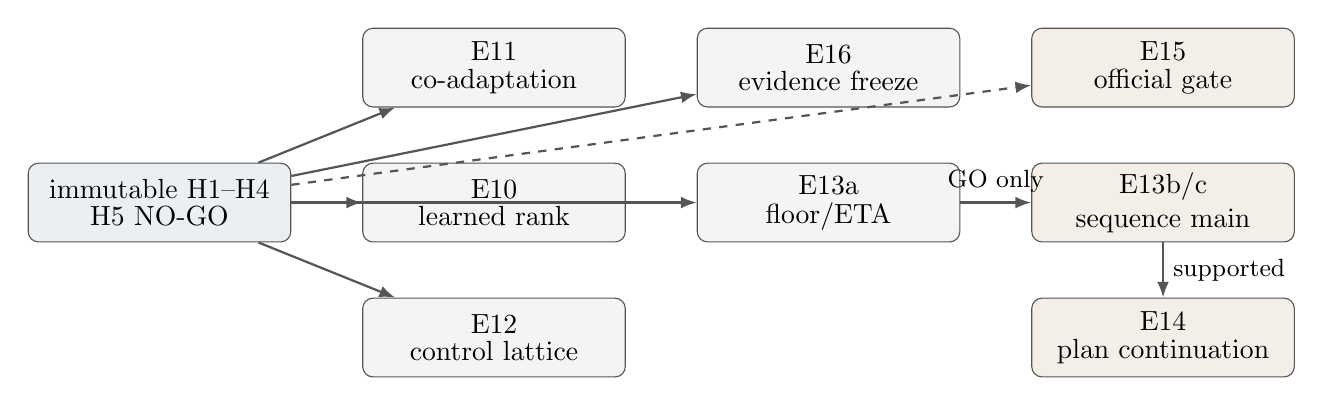
\begin{tikzpicture}[
 node distance=7mm and 9mm,
 n/.style={draw=Line,rounded corners=1.3mm,fill=Panel,minimum width=33mm,minimum height=10mm,text width=31mm,align=center},
 c/.style={draw=Line,rounded corners=1.3mm,fill=Core,minimum width=33mm,minimum height=10mm,text width=31mm,align=center},
 f/.style={draw=Line,rounded corners=1.3mm,fill=Future,minimum width=33mm,minimum height=10mm,text width=31mm,align=center},
 a/.style={-{Latex[length=2mm]},thick,draw=Line}
]
\node[c] (core) {\shortstack{immutable H1--H4\\H5 NO-GO}};
\node[n,right=of core] (e10) {\shortstack{E10\\learned rank}};
\node[n,above=of e10] (e11) {\shortstack{E11\\co-adaptation}};
\node[n,below=of e10] (e12) {\shortstack{E12\\control lattice}};
\node[n,right=of e10] (e13a) {\shortstack{E13a\\floor/ETA}};
\node[f,right=of e13a] (e13b) {\shortstack{E13b/c\\sequence main}};
\node[f,below=of e13b] (e14) {\shortstack{E14\\plan continuation}};
\node[n,above=of e13a] (e16) {\shortstack{E16\\evidence freeze}};
\node[f,above=of e13b] (e15) {\shortstack{E15\\official gate}};
\draw[a] (core)--(e10);\draw[a] (core)--(e11);\draw[a] (core)--(e12);\draw[a] (core)--(e13a);\draw[a] (core)--(e16);\draw[a,dashed] (core)--(e15);
\draw[a] (e13a)--node[above,font=\small]{GO only}(e13b);
\draw[a] (e13b)--node[right,font=\small]{supported}(e14);
\end{tikzpicture}
\caption{E10, E11, E12, E13a와 E16은 즉시 독립 실행 가능하다. E13b와 E14만 hard dependency를 갖는다.}
\end{figure}

\subsection{지금 즉시 실행하는 4개 GPU lane}
\begin{center}
\begin{tabularx}{\textwidth}{c l X l}
\toprule
GPU & 실험 & 핵심 질문 & 의존성 \\
\midrule
0 & E10 & learned rank가 best-rank floor를 추적하는가 & 없음 \\
1 & E11 & representation 학습 후에도 noncommuting obstruction이 남는가 & 없음 \\
2 & E12 & architecture freedom이 필요한 demand에서만 선택적 이득인가 & 없음 \\
3 & E13a & structured sequence floor, tied-dual gap과 actual ETA가 성립하는가 & 없음 \\
CPU & E16 & 기존 evidence report와 hash 동결 & 없음 \\
\bottomrule
\end{tabularx}
\end{center}

실행 명령은 다음과 같다.
\begin{verbatim}
bash scripts/launch_postcore_wave1.sh /home/minjun_dev/CATENA

python experiments/e16_core_evidence_freeze.py \
  --config configs/e16_core_evidence_freeze.yaml \
  --device cpu \
  --artifact-root /data/minjun_dev/CATENA/artifacts
\end{verbatim}

E13a GO 후에만 \texttt{launch\_sequence\_if\_go.sh}를 사용한다. E13c가 supported가 아니면 E14를 실행하지 않는다.

\subsection{예상 계산량과 중단 규칙}
정확한 GPU-hour는 E13a의 실측 throughput을 우선한다. 현재 계획상 상대적인 범위는 다음과 같다.

\begin{center}
\begin{tabular}{lrrl}
\toprule
Stage & 예상 GPU-hours & 병렬 wall-clock & 중단 조건 \\
\midrule
E10 & 20--60 & 0.5--1.5일 & rank-error 단조성 실패 \\
E11 & 20--60 & 0.5--1.5일 & common rotation 회복 실패 \\
E12 & 40--100 & 1--3일 & selective interaction 또는 NI 실패 \\
E13a & 2--10 & 수 시간 & floor/gain/retention/throughput 중 하나 실패 \\
E13b/c & 150--450 & 2--6일 & E13a NO-GO 또는 seed 방향 불안정 \\
E14 & 10--40 & 수 시간--1일 & E13c unsupported \\
E15 & 환경 의존 & 별도 & pin/parity 실패 \\
\bottomrule
\end{tabular}
\end{center}

E10--E12가 모두 null이어도 REALM core는 손상되지 않는다. E13a가 NO-GO이면 sequence experiment를 중단하고 그 failure를 설계 경계로 기록한다.

\section{실험 결과별 허용 주장}
\begin{longtable}{p{32mm}p{55mm}p{58mm}}
\toprule
실험 결과 & 허용 주장 & 금지 주장 \\
\midrule
E10 rank threshold 추적 & registered smooth family에서 learned control rank가 intrinsic demand rank와 함께 증가 & pretrained LM의 universal minimal rank \\
E10 error만 단조 감소 & richer rank의 capacity benefit & demand algebra가 rank를 정량 예측 \\
E11 predicted pattern & representation co-adaptation 후에도 noncommuting family는 richer control을 요구 & representation learning이 어떤 task에서도 diagonal limitation을 제거하지 못함 \\
E12 selective lattice & 추가 freedom은 그것을 요구하는 demand에서만 이득 & 특정 architecture의 보편 우월성 \\
E13c supported & structured event sequence에서 repeated update의 dual-control advantage & 자연어, agent, official GDN2 transfer \\
E14 supported & tested structured plan state의 one-time repair와 retention & general planning, production break-even \\
E15 PASS & pinned official implementation의 numerical readiness & official backend에서 task performance 우위 \\
\bottomrule
\end{longtable}

\section{워크숍 제출과 top-tier 확장}
\subsection{REALM short paper}
REALM은 4쪽 short paper에서 작은 집중 기여와 negative result를 허용한다\citep{realm2026}. 제출 본문의 core는 다음으로 고정한다.

\begin{enumerate}
\item H1: bounded behavioral reachability calibration;
\item E02b: erase/write magnitude factorization;
\item E03b: joint-diagonalization calibration;
\item H4: functional mediation;
\item H5 NO-GO: semantic front-end factorization의 boundary.
\end{enumerate}

E10--E12 또는 E13 pilot은 결과가 깨끗하고 한 panel로 설명될 때만 추가한다. 그렇지 않으면 workshop 뒤 full paper로 이동한다. H6 multi-update 전체, official KVEraser Pareto, broad recurrent-vs-Transformer superiority는 이번 short paper의 main claim이 아니다.

\subsection{Top-tier full paper}
Post-core가 성공하면 논문의 중심은 다음으로 확장된다.

\begin{claimbox}
\textbf{Transactional Control Algebra principle.} Update-demand family가 생성하는 algebra의 rank, joint diagonalizability, address structure와 state dependence가, 그 family를 낮은 error로 실현하는 최소 memory-control architecture를 결정한다.
\end{claimbox}

Full paper는 다음 네 층을 포함한다.
\begin{enumerate}
\item analytic/controlled geometry: 현재 H1--H4;
\item learned operator and representation: E10--E12;
\item repeated sequence persistence: E13--E14;
\item official recurrent/KV-cache boundary: E15 이후 matched replication.
\end{enumerate}

장기적으로 external explicit world state와 dense predictive belief를 연결하려면 semantic demand inference뿐 아니라 action-conditioned future prediction이 추가되어야 한다. 현재 연구는 world model 자체가 아니라 그 전제인 \textbf{low-latency, geometry-matched belief assimilation primitive}를 구축한다.

\section{Repository와 실행 계약}
각 실험은 Python entry point 하나와 YAML config 하나에 대응한다.

\begin{center}
\begin{tabularx}{\textwidth}{l l X}
\toprule
Stage & Entry point & 핵심 artifact \\
\midrule
E10 & \texttt{e10\_learned\_rank\_scaling.py} & \texttt{rank\_scaling\_metrics.jsonl} \\
E11 & \texttt{e11\_representation\_control\_coadaptation.py} & \texttt{coadaptation\_metrics.jsonl} \\
E12 & \texttt{e12\_control\_algebra\_lattice.py} & \texttt{control\_lattice\_metrics.jsonl} \\
E13a & \texttt{e13a\_sequence\_floor\_throughput.py} & calibration metrics/checkpoints \\
E13b & \texttt{e13b\_transactional\_sequence\_memory.py} & per-seed checkpoint/main metrics \\
E13c & \texttt{e13c\_transactional\_sequence\_aggregate.py} & paired aggregate \\
E14 & \texttt{e14\_plan\_continuation.py} & plan-continuation metrics \\
E15 & \texttt{e15\_official\_backend\_gate.py} & pinned backend rows \\
E16 & \texttt{e16\_core\_evidence\_freeze.py} & evidence registry/results macros \\
\bottomrule
\end{tabularx}
\end{center}

Artifact root는 \texttt{/data/minjun\_dev/CATENA/artifacts}로 고정한다. Dry-run과 main은 별도 run directory를 만들며, 기존 report는 사후 편집하지 않는다. E15는 official plugin이 없을 때 reference fallback을 하지 않는다. Codex는 \texttt{CODEX\_POSTCORE.md}, dependency DAG, artifact contract와 experiment-specific docs를 먼저 읽어야 한다.

\section{최종 판단}
현재 controlled core는 매우 깨끗하지만 oracle candidate/address를 사용하는 analytic setting이라는 한계를 갖는다. 남은 GPU를 같은 geometry에서 seed를 더 늘리는 데 사용하는 것은 연구의 ceiling을 올리지 못한다. 가장 가치 있는 다음 단계는 다음 순서다.

\begin{enumerate}
\item \textbf{E10}: oracle low-rank 가능성을 learned rank requirement로 전환;
\item \textbf{E11}: representation co-adaptation 반론을 제거;
\item \textbf{E12}: 최근 recurrent architecture freedom을 하나의 demand lattice로 정렬;
\item \textbf{E13--E14}: single-step geometry를 repeated sequence와 stale plan repair로 연결;
\item \textbf{E15}: official implementation에서 수치 및 behavior contract를 검증.
\end{enumerate}

이 연구 프로그램의 고점은 새로운 gate 하나를 더 제안하는 데 있지 않다. 목표는 다음의 일반 원리를 empirical design map으로 만드는 것이다.
\[
\boxed{
\text{The geometry and algebra of update demands determine the minimal memory-control architecture.}
}
\]

\printbibliography
\end{document}
